\documentclass[12pt,a4paper]{article}
\usepackage{geometry}
\geometry{left=2.54cm, right=2.54cm, top=2.98cm, bottom=2.98cm}
\usepackage{fancyhdr} 
\usepackage{enumerate}
\usepackage{graphicx}
\usepackage{subfigure}
\usepackage{caption}
\usepackage{float}
\usepackage{indentfirst}
\usepackage{threeparttable}
\usepackage{longtable}
\usepackage{hyperref}
\usepackage{setspace}
\usepackage{amsmath}
\hypersetup{
	colorlinks=true,
	linkcolor=black,
	filecolor=black,      
	urlcolor=black,
	citecolor=black,
}
\title{Newton's Second Law}
\author{ZHANGYIHENG 10.7 27}
\date{}
\linespread{1.25}
\begin{document}
\maketitle
\tableofcontents
\newpage
\section{Introduction}
\subsection{Definition of Newton's Second Law}
Newton's Second Law of Motion states that when a force is applied to a body, the acceleration of a body is proportional to the force applied and inversely proportional to its mass.
\subsection{Aim of the Experiment}
The goal of the investigation is to validate Newton's second law of motion to by finding the relationship between the acceleration(denoted by $a$) and external force(denoted by $F$) as well as the relationship between acceleration and the total mass of the system(denoted by $m$).\par
To achieve our objective, we will conduct a series of experiments using different masses and forces. By analyzing the data obtained, we will determine whether the acceleration of a body is proportional to the force acting on it and inversely proportional to its mass, so as to examine the fundamental physics principal. \par
\subsection{Equipments Used}
\begin{enumerate}
    \setlength{\itemsep}{0em}
    \setlength{\parsep}{0em}
    \item air track
    \item air pump
    \item light gats
    \item digital timer
    \item glider
    \item weights
    \item little buckets and string
    \item digital balance
    \setlength{\topsep}{0em}
\end{enumerate}

\section{Procedure}
\subsection{Data Collecting}
To begin our experiment, we started by measuring the weight of all our apparatuses. We carefully weighed the mass of the glider as well as the mass of the bucket that we used to add screws to. This initial step was crucial as it allowed us to calculate the force acting on the glider, which is an essential component of our experiment. \par
Next, we turned on the air pump and placed the glider on the air track. We experimented several times, changing the number of screws in the bucket to alter the drag force acting on the glider. We collected data each time by using light gates to measure the acceleration of the glider. All the data with uncertainty are recorded in the data table with appendix.\par
\subsection{Data Processing}
\subsubsection{Tension on the Glider}
After completing the measurement process, we obtained the mass of the glider, which was determined to be 18.87$\pm 0.01 $$g$.\par
Using Newton's Second Law, we know that
\[
    \left\{\begin{matrix} 
        Mg - T = Ma \\
        T = ma
      \end{matrix}\right. 
\]
in which $ m $ represent the mass of the glider and $ M $ represent the mass of the weight. Simplify the equation above we know $\displaystyle{T = G \times \frac{m}{m + M} }$.
Take data set 1 for example, we have $ G = mg = 7.9 \times 9.81 \approx 0.0775N $ and $ T = 0.0775 \times \displaystyle{\frac{188.7}{188.7 + 7.9}} \approx = 0.0744 N $.

\subsubsection{Uncertainty of the Tension}
Next we'll determine the uncertainty of our processed data.
\[
    \%\Delta T = (\frac{\Delta G}{G} + \frac{\Delta m}{m} + \frac{\Delta M+m}{M+m}) \times 100\% 
\]
\[
    \Delta T = \% \Delta T \times T
\]
In the case above when $ m = 7.2g $, $ \Delta T \approx 0.001 N$.
All the other $ T $ are calculated and recorded in the data table.
\subsubsection{Further analysis}
Further analysis of the data revealed that the acceleration of the glider increased as the magnitude of the external force acting on it increased. To better understand this relationship, we used Logger Pro to create a graph of the data points. After using linear fit, we can see the relationship between $ T $ and $ a $ is $ T = 5.63 \times 10^ {-4} + 0.0664N$.\par
\section{Conclusion and Evaluation}
\subsection{Conclusion}
Based on our analysis of the data and the gradient of the line in the graph plotted using Logger Pro, we estimate that the mass of the glider used in our experiment is approximately $ 5.63 \times 10^ {-4}  $.\par
\subsection{Evaluation}
Based on the measurement before, it appears that the actual mass of the glider is actually 188.7$g$, which is very different from the value we calculated earlier.\par
Besides, Tension is not actually proportional to the Acceleration. From the graph we can know that, only when tension is over $ 0.07N $ can the glider began to move, indicating a systematic error in my experiment.\par
This discrepancy may be due to various factors such as measurement errors, environmental factors, or other sources of uncertainty. It is important to consider these factors when next time we do perform our investigation. Below are their corresponding solutions that may reduce the impact they have on our results.\par
\textbf{Measurement errors}: The mass of the glider may not have been measured accurately due to errors in the measurement process, such as incorrect use of the weighing scale or imprecise readings. The inaccuracy could be also due to the light gates's uncertainty. To minimize these errors, we can repeat the measurements multiple times and calculate an average value. We can also use a more precise measuring apparatuses to ensure the precision.\par
\textbf{Environmental factors}: The air track may not have been perfectly level, which could have affected the acceleration of the glider and thus its mass calculation. To address this issue, we can carefully level the air track next time and ensure that it is stable and secure during the experiment.\par
\textbf{Friction}: There may have been some friction between the glider and the air track, which could have affected its acceleration and mass calculation. To reduce friction, we can ensure that the air track is clean and horizontal and free from any debris or dust. We can also use a lubricant to further reduce friction.\par
\textbf{Air resistance}: The glider may have experienced air resistance during its motion, which could have affected its acceleration and thus its mass calculation. To minimize air resistance, we can use a more streamlined shape for the glider or reduce the speed of the air flow in the air track.\par
By taking these factors into consideration and implementing the corresponding solutions, we can probably reduce the sources of uncertainty in our experiment and obtain more accurate and reliable results.\par
% \newpage
\section{Appendix}
\subsection{Tables}
\subsubsection*{Raw Data Table}
\begin{table}[!ht]
    \centering
    \caption{Processed Data Table}
    \begin{tabular}{|c|c|c|c|c|c|c|c|c|}
    \hline
        M (g) & m (g) & $ \Delta m $ & G (N) & $ \Delta G $& T($ N $) & $ \Delta T $& $ a  (ms) $ & $ \Delta a $\\ \hline
        188.7 & 12.4 & ±0.1 & 0.122& 0.001& 0.114& 0.001 & 84.1 & 0.1  \\ \hline
        188.7 & 11.7 & 0.1 & 0.115& 0.001& 0.108& 0.001 & 78.4 & 0.1  \\ \hline
        188.7 & 10.9 & 0.1 & 0.107& 0.001& 0.101& 0.001 & 60.5 & 0.1  \\ \hline
        188.7 & 10.2 & 0.1 & 0.100& 0.001& 0.0949& 0.001 & 44.2 &0.1  \\ \hline
        188.7 & 9.4 & 0.1 & 0.0922& 0.001& 0.0878& 0.001 & 37.9 & 0.1  \\ \hline
        188.7 & 8.6 & 0.1 & 0.0844& 0.001& 0.0807& 0.001 & 26.4 & 0.1  \\ \hline
        188.7 & 7.9 & 0.1 & 0.0775& 0.001& 0.0744& 0.001 & 17.3 & 0.1 \\ \hline
    \end{tabular}
\end{table}

\subsection{Figures}
Here are pictures of equipments and some of the process of the experiments.
\begin{figure}[h]
    \centering
    \subfigure[Air Pump]{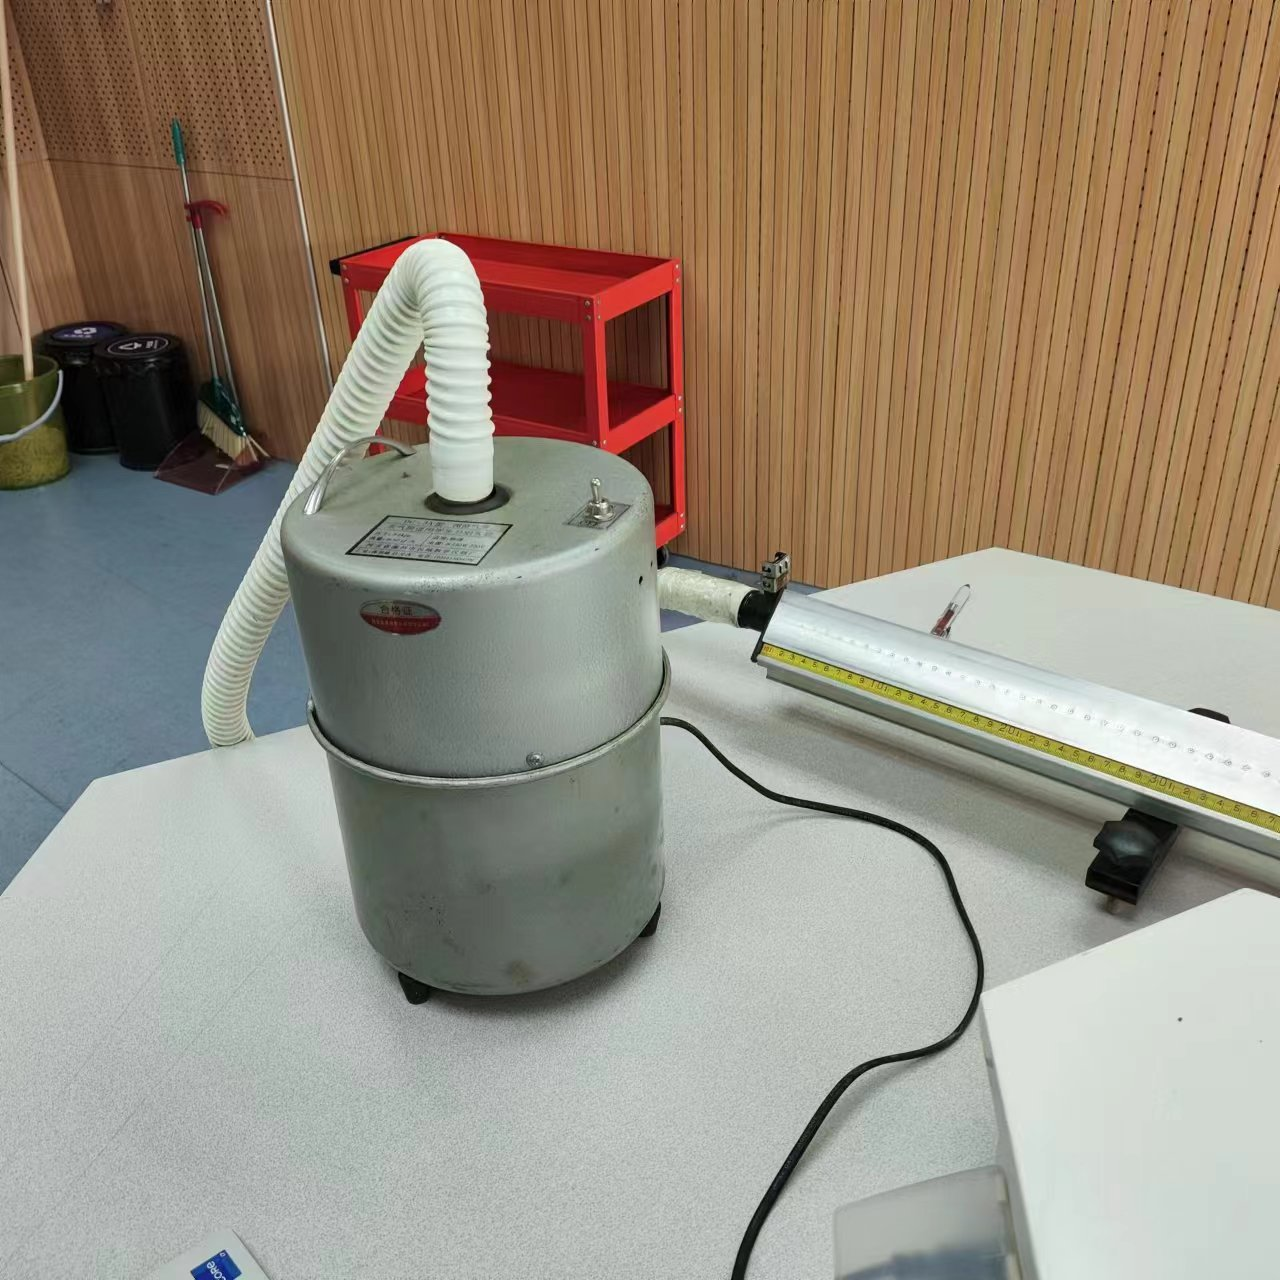
\includegraphics[width=0.3\textwidth]{airpump.jpeg}}
    \subfigure[Glider]{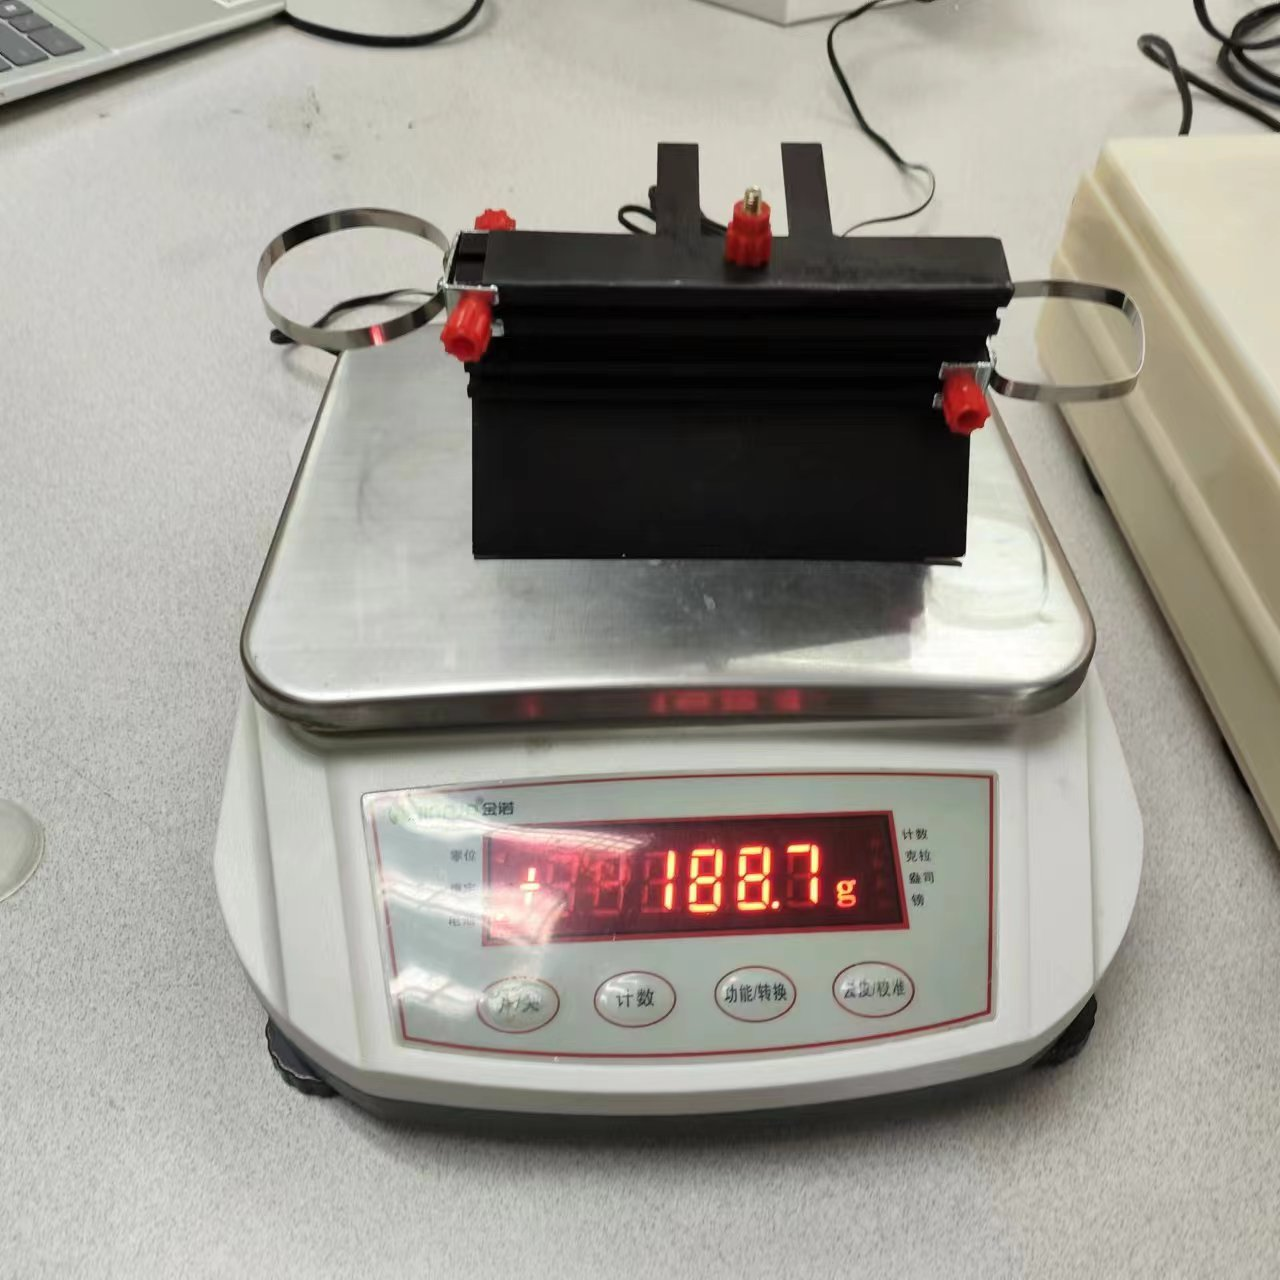
\includegraphics[width=0.3\textwidth]{glider.jpeg}}
    \subfigure[Air Track]{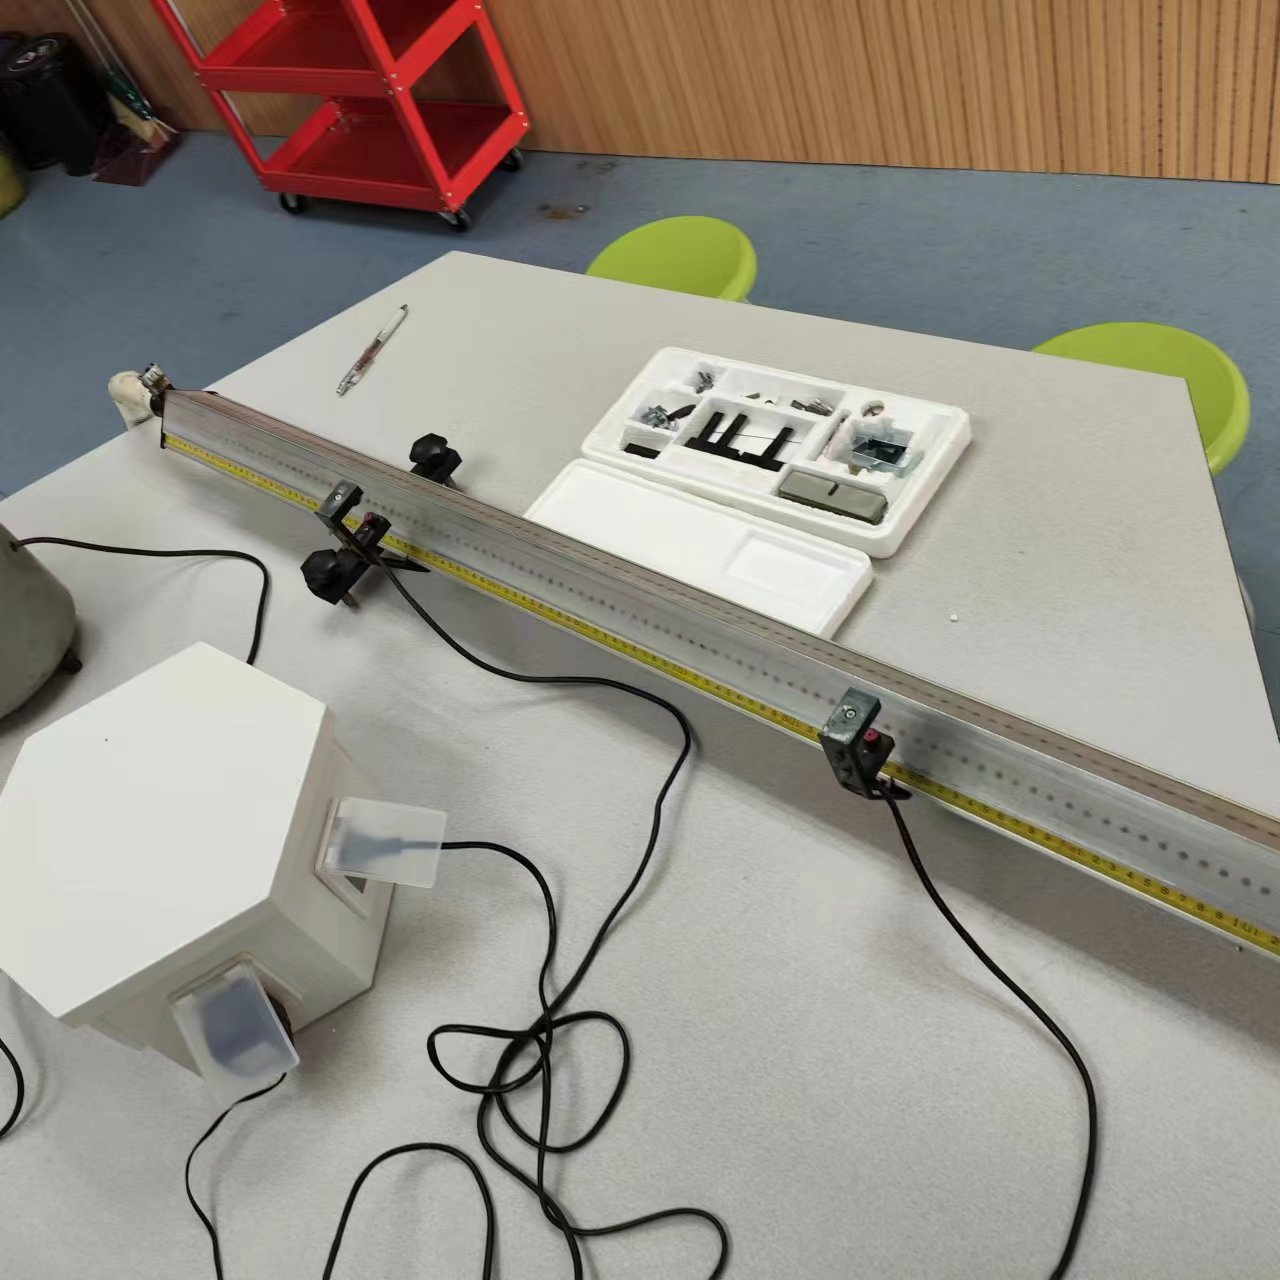
\includegraphics[width=0.3\textwidth]{airtrack.jpeg}}
    \caption{Equipments}
    \vspace{-0.5cm}
\end{figure}
\begin{figure}[h]
    \centering
    \subfigure[Weight1]{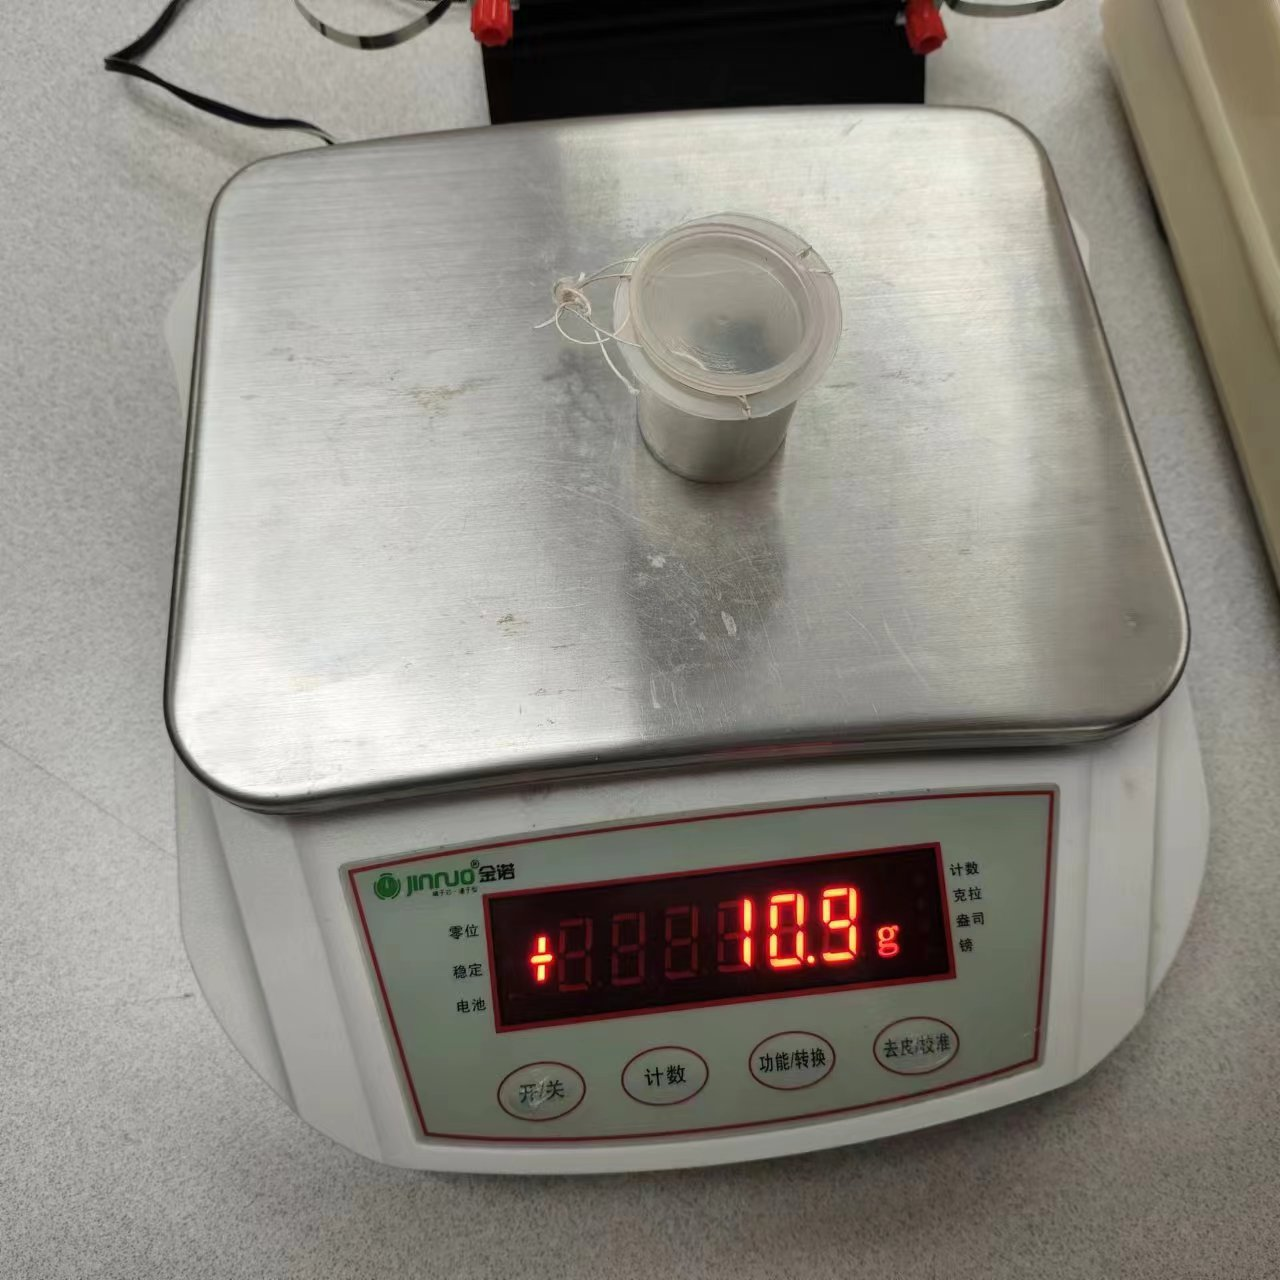
\includegraphics[width=0.45\textwidth, height = 6cm]{bucket1.jpeg}}
    \subfigure[Weight2]{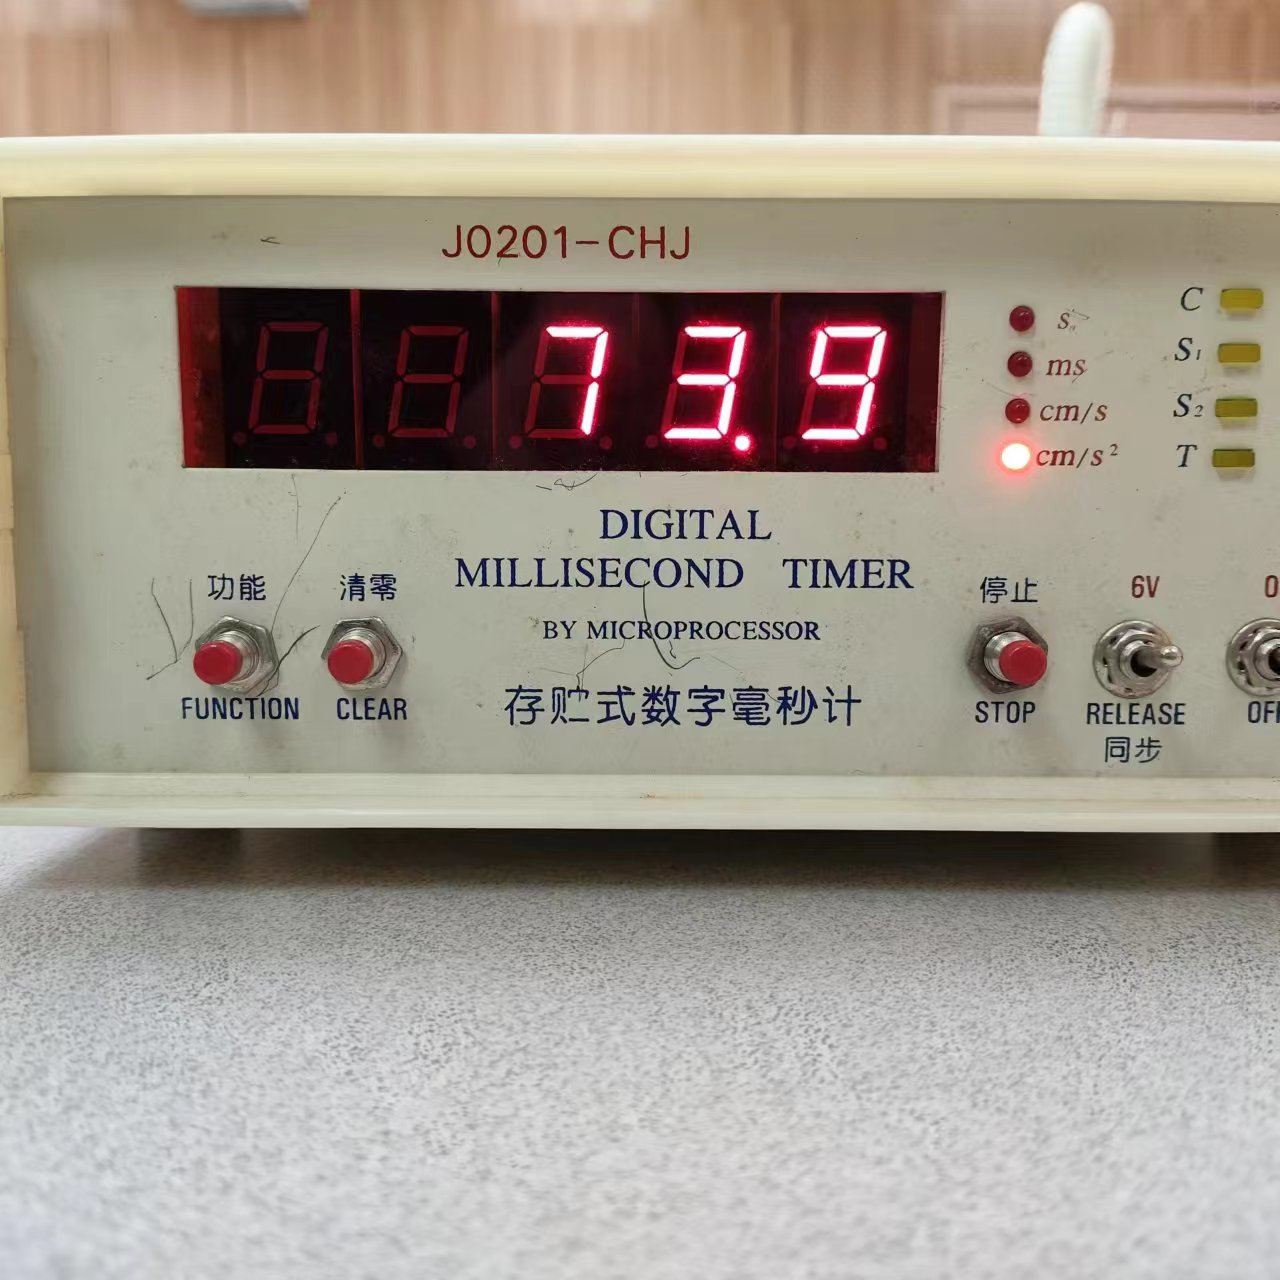
\includegraphics[width=0.45\textwidth, height = 6cm]{acc2.jpeg}}
    \caption{Measuring Mass of the Bucket and the Acceleration}
    \vspace{-0.5cm}
\end{figure}
\subsection{Graphs}
\begin{figure}[H]
    \centering
    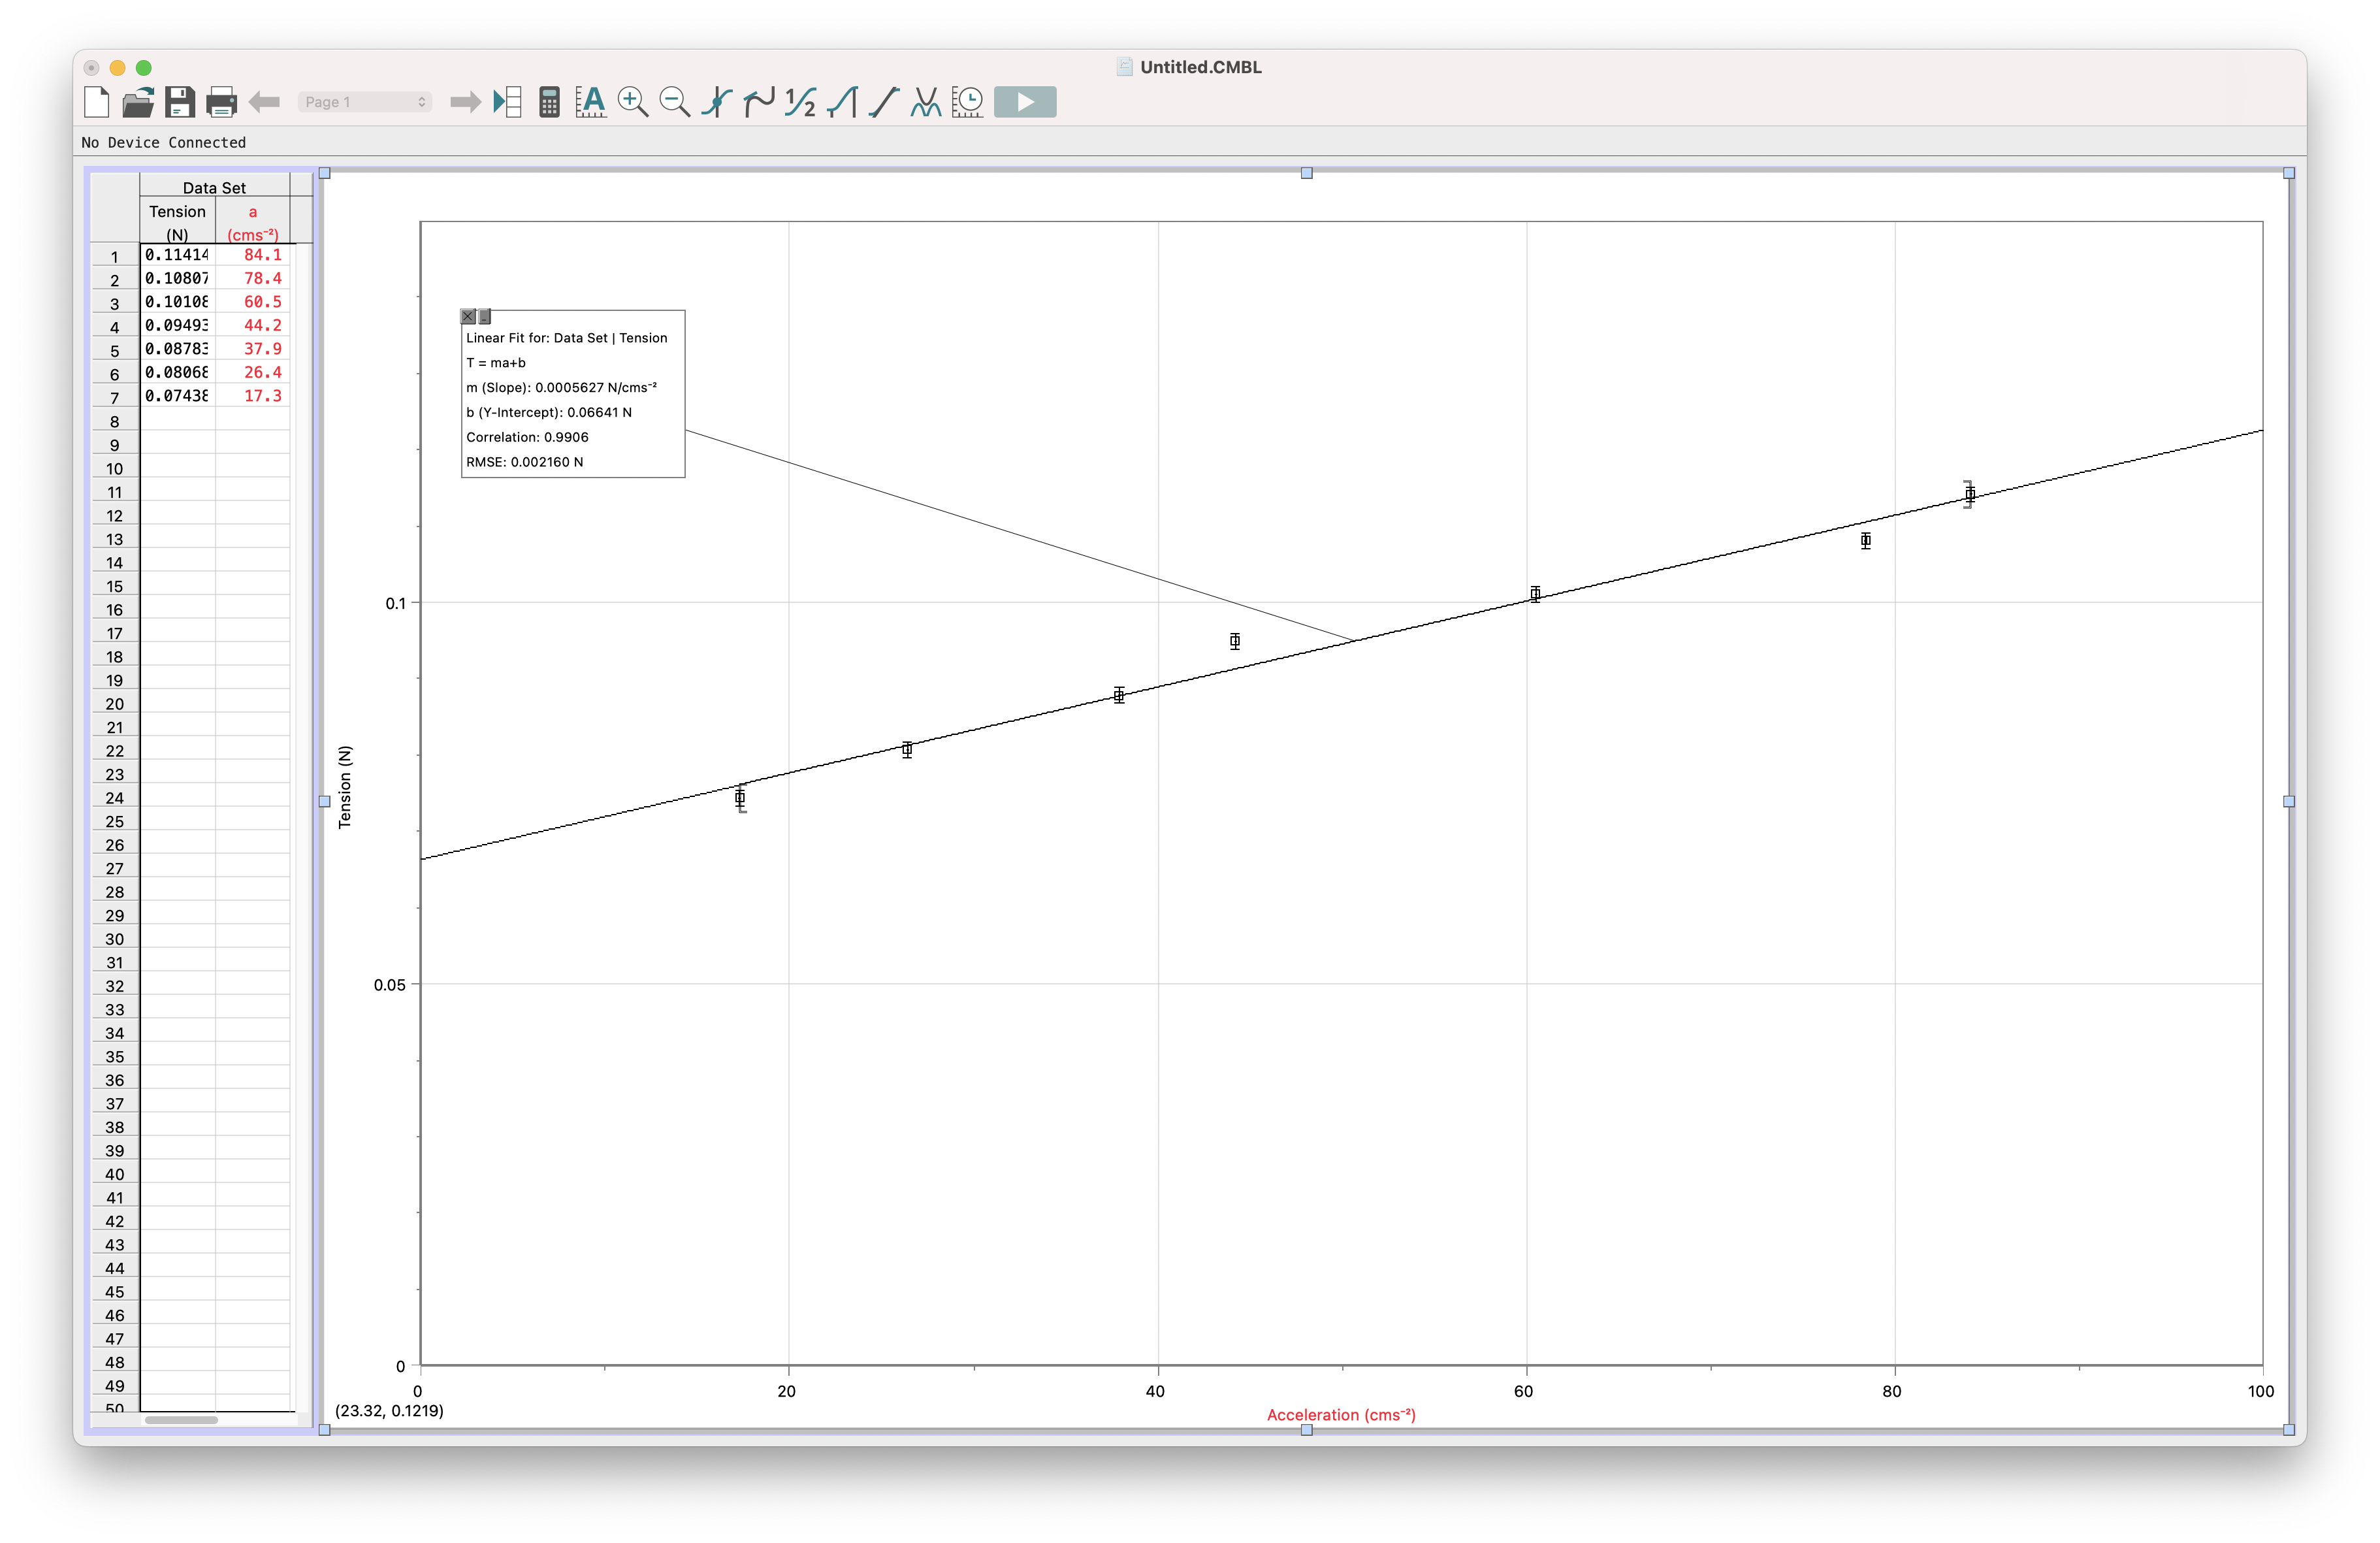
\includegraphics[width=15.9cm, height=9.8cm]{F-a.png}
    \caption{$F-a$ Graph}
\end{figure}
\end{document}